\chapter{Clustering and Embedding}
Instead of finding interesting projections from data, we can use clustering algorithms to find groups or categories of the data. Each cluster is represented by a prototype $\boldsymbol{w}$.

Given set of $\boldsymbol{x}^{(\alpha)}, \alpha=1,\dots,p;  \boldsymbol{x}^{(\alpha)} \in \mathbb{R}^N$, we want to assign them into $M$ clusters where the indicator

\begin{align*}
	m_q^{(\alpha)} = \begin{cases}
    1,& \text{if } \boldsymbol{x}^{(\alpha)} \in \text{cluster} \ q\\
    0,              & \text{otherwise}
\end{cases}
\end{align*}
and $\sum_q m_q^{(\alpha)} = 1 $.

\section{K-Means Clustering}
\subsection{Cost function}
$$
E^T_{[ \{ m_q^{(\alpha)} \}, \{ \boldsymbol{w}_q \}]} = \frac{1}{p}\sum_{\alpha, q} m_q^{(\alpha})\bigg(  \boldsymbol{x}^{(\alpha)} - \boldsymbol{w}_q \bigg)^2
$$

\begin{itemize}
	\item Cluster center is defined by continuous variable
	\item Cluster assign is binary 
	\item Dissimilarity is measured by Euclidean distance.
\end{itemize}

\begin{algorithm}[H]
\caption{Batch K-means}
 \KwData{$\boldsymbol{w}_q = \langle \boldsymbol{x} \rangle + \boldsymbol{\eta}_q$ where $\boldsymbol{\eta}_q$ is a random vector}
 \While{ not converge}{
  $\forall \alpha \in p : m_q^{(\alpha)} = 1 \Bigg \{ q = \underset{\gamma}{\text{argmin}} \bigg( \boldsymbol{x}^{(\alpha)} - \boldsymbol{w}_\gamma \bigg) ^ 2 \Bigg \}$  \\
  
  $\forall q \in M : \boldsymbol{w}_q = \frac{\sum_\alpha m_q^{(\alpha)} \boldsymbol{x}^{(\alpha)}}{\sum_\alpha m_q^{(\alpha)}}$ 
 }
\end{algorithm}

\begin{itemize}
	\item $E^T$ is monotonic decreasing.
	\item $\boldsymbol{w}_q$ is center of mass $\rightarrow$ $E^T$ is total variance.
\end{itemize}

\begin{algorithm}[H]
\caption{Online K-means}
 \KwData{$\boldsymbol{w}_q = \langle \boldsymbol{x} \rangle + \boldsymbol{\eta}_q$ where $\boldsymbol{\eta}_q$ is a random vector}
 \KwData{$\epsilon \in [0,1] $}
 \While{not converge}{
 Select a point $\boldsymbol{x}^{(\alpha)}$ \\
 $ q \leftarrow \underset{\gamma}{\text{argmin}} \bigg( \boldsymbol{x}^{(\alpha)} - \boldsymbol{w}_\gamma \bigg) ^ 2 $ \\
 $\boldsymbol{w}_q \leftarrow \boldsymbol{w}_q + \epsilon ( \boldsymbol{x}^{(\alpha)} - \boldsymbol{w}_q)$
 }
\end{algorithm}

\begin{figure}[hbt]
	\center
  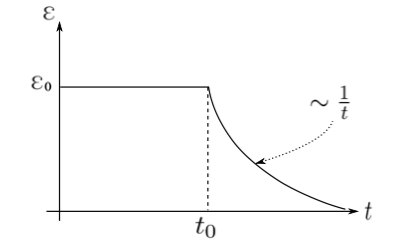
\includegraphics[width=0.5\textwidth]{figures/cl-annealing-epsilon}
  \caption{$\epsilon$ Annealing Schedule }
  \label{fig:cl-annealing-epsilon}
\end{figure}

\subsection{Number of prototypes}
\begin{itemize}
	\item $E^T \propto \frac{1}{M}$
	\item $E^T = 0$ when $M = p$
\end{itemize}

\begin{algorithm}[H]
\caption{Iterative refinement}
 \KwData{$\boldsymbol{w}_q = \frac{1}{p} \sum_\alpha \boldsymbol{x}^{(\alpha)} $}
 \KwData{$ (E^T)^* =$ some constant}
 \KwData{$M = 1 $}
 \While{$E^T > (E^T)^*$}{
	$$q \leftarrow \underset{\gamma \in M}{\text{argmax}} \frac{\sum_\alpha m_\gamma^{(\alpha)}(\boldsymbol{x}^{(\alpha)} - \boldsymbol{w}_q)^2 }{\sum_\alpha m_\gamma^{(\alpha)}}$$
	
	$\boldsymbol{w}_{M+1} \leftarrow \boldsymbol{w}_q + n_q$ \\
	$M \leftarrow M+1$ \\
	do regular K-Means algorithm with $M$ prototypes
% Select a point $\boldsymbol{x}^{(\alpha)}$ \\
% $ q \leftarrow \underset{\gamma}{\text{argmin}} \bigg( \boldsymbol{x}^{(\alpha)} - \boldsymbol{w}_\gamma \bigg) ^ 2 $ \\
% $\boldsymbol{w}_q \leftarrow \boldsymbol{w}_q + \epsilon ( \boldsymbol{x}^{(\alpha)} - \boldsymbol{w}_q)$
 }
\end{algorithm}

\subsection{Validation Measure}
Given $Y = (y_1, ..., y_p), y_i \in \{1,..,M\}$ solution of the clustering algorithm. We can measure the solutions $Y_1, Y_2$ by 
$$
d = \frac{1}{|Y_1|} \sum_\alpha \boldsymbol{1}\{ Y_{1,\alpha} \ne Y_{2,\alpha} \}
$$


\begin{figure}[hbt]
	\center
	% TODO What does phi(x) means?
  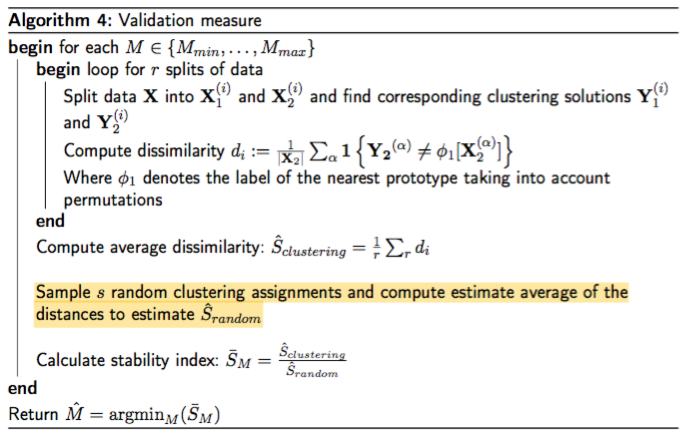
\includegraphics[width=0.5\textwidth]{figures/cl-validation-measure}
  \caption{Validation measure}
\end{figure}



\section{Pairwise Clustering}
\textit{distance matrix} $\{ d_{\alpha \alpha'} \}$ represents pairwise data and it is symmetric and its on diagonal elements are zero.

\subsection{Cost Function}
\begin{align*}
	E_{ [ \{  m_q^{(\alpha)} \}] } &= \frac{1}{2p} \sum_q \frac{ \sum_{\alpha \alpha'} m_q^{(\alpha)} m_q^{(\alpha')} ( \boldsymbol{x}^{(\alpha)} - \boldsymbol{x}^{(\alpha')})^2  }{\sum_\alpha m_q^{(\alpha)} } \\
	&= \frac{1}{2p} \sum_q \frac{ \sum_{\alpha \alpha'} m_q^{(\alpha)} m_q^{(\alpha')} \bigg ( (\boldsymbol{x}^{(\alpha)})^2 - 2(\boldsymbol{x}^{(\alpha)})^T\boldsymbol{x}^{(\alpha')} + (\boldsymbol{x}^{(\alpha')})^2 \bigg )  }{\sum_\alpha m_q^{(\alpha)} } \\
	&= \frac{1}{2p} \sum_q \frac{ \sum_{\alpha \alpha'} m_q^{(\alpha)} m_q^{(\alpha')}  (\boldsymbol{x}^{(\alpha)})^2 
	}{\sum_\alpha m_q^{(\alpha)} } - 2 \frac{ \sum_{\alpha \alpha'} m_q^{(\alpha)} m_q^{(\alpha')}  \boldsymbol{x}^{(\alpha)}\boldsymbol{x}^{(\alpha')}
	}{\sum_\alpha m_q^{(\alpha)} } + \frac{ \sum_{\alpha \alpha'} m_q^{(\alpha)} m_q^{(\alpha')}  (\boldsymbol{x}^{(\alpha')})^2 
	}{\sum_\alpha m_q^{(\alpha)} } \\
	&= \frac{1}{2p} \sum_q \frac{ \sum_{\alpha} m_q^{(\alpha)} (\boldsymbol{x}^{(\alpha)})^2  \sum_{\alpha'} m_q^{(\alpha')}  
	}{\sum_\alpha m_q^{(\alpha)} } - 2 \frac{ \sum_{\alpha} m_q^{(\alpha)} \boldsymbol{x}^{(\alpha)} \sum_{\alpha'} m_q^{(\alpha')}  \boldsymbol{x}^{(\alpha')}
	}{\sum_\alpha m_q^{(\alpha)} } + \frac{ \sum_{\alpha} m_q^{(\alpha)} (\boldsymbol{x}^{(\alpha)})^2  \sum_{\alpha'} m_q^{(\alpha')}  
	}{\sum_\alpha m_q^{(\alpha)} } \\
	&= \frac{1}{2p} \sum_q \sum_{\alpha} m_q^{(\alpha)} (\boldsymbol{x}^{(\alpha)})^2  
- 2 \sum_{\alpha} m_q^{(\alpha)} x^{(\alpha)} \frac{  \sum_{\alpha'} m_q^{(\alpha')}  \boldsymbol{x}^{(\alpha')}
	}{\sum_{\alpha'} m_q^{(\alpha')} } + \sum_{\alpha} m_q^{(\alpha)} (\boldsymbol{x}^{(\alpha)})^2   \\
	&= \frac{1}{p} \sum_q \sum_{\alpha} m_q^{(\alpha)} (\boldsymbol{x}^{(\alpha)})^2  
-  \sum_{\alpha} m_q^{(\alpha)} (\boldsymbol{x}^{(\alpha)})^T \boldsymbol{w}_q \\
&= \frac{1}{p} \Bigg \{  \sum_{q, \alpha} m_q^{(\alpha)}  (\boldsymbol{x}^{(\alpha)})^2  
-   \sum_{q} \sum_{\alpha}m_q^{(\alpha)}  (\boldsymbol{x}^{(\alpha)})^T \boldsymbol{w}_q  \Bigg \}\\
&= \frac{1}{p} \Bigg \{  \sum_{q, \alpha} m_q^{(\alpha)}  (\boldsymbol{x}^{(\alpha)})^2  
-   \sum_{q} \sum_{\alpha}m_q^{(\alpha)} (\boldsymbol{x}^{(\alpha)})^T  \boldsymbol{w}_q  -  \sum_{q} \sum_{\alpha}m_q^{(\alpha)} \boldsymbol{w}_q^T \boldsymbol{w}_q  + \sum_{q} \sum_{\alpha}m_q^{(\alpha)} \boldsymbol{w}_q^T \boldsymbol{w}_q \Bigg \} \\
&= \frac{1}{p} \Bigg \{  \sum_{q, \alpha} m_q^{(\alpha)}  (\boldsymbol{x}^{(\alpha)})^2  
-   \sum_{q} \sum_{\alpha}m_q^{(\alpha)} (\boldsymbol{x}^{(\alpha)})^T  \boldsymbol{w}_q  -  \sum_{q} \sum_{\alpha}m_q^{(\alpha)} \frac{  \sum_{\alpha'} m_q^{(\alpha')}  (\boldsymbol{x}^{(\alpha')})^T
	}{\sum_{\alpha'} m_q^{(\alpha')} } \boldsymbol{w}_q  + \sum_{q} \sum_{\alpha}m_q^{(\alpha)} \boldsymbol{w}_q^T \boldsymbol{w}_q \Bigg \} \\
&= \frac{1}{p} \Bigg \{  \sum_{q, \alpha} m_q^{(\alpha)}  (\boldsymbol{x}^{(\alpha)})^2  
-   \sum_{q} \sum_{\alpha}m_q^{(\alpha)} (\boldsymbol{x}^{(\alpha)})^T  \boldsymbol{w}_q  -  \sum_{q} \frac{\sum_{\alpha}m_q^{(\alpha)}}{\sum_{\alpha'} m_q^{(\alpha')}}  \sum_{\alpha'} m_q^{(\alpha')}  (\boldsymbol{x}^{(\alpha')})^T
	\boldsymbol{w}_q  + \sum_{q} \sum_{\alpha}m_q^{(\alpha)} \boldsymbol{w}_q^T \boldsymbol{w}_q \Bigg \} \\
	&= \frac{1}{p} \Bigg \{  \sum_{q, \alpha} m_q^{(\alpha)}  (\boldsymbol{x}^{(\alpha)})^2  
-   \sum_{q} \sum_{\alpha}m_q^{(\alpha)} (\boldsymbol{x}^{(\alpha)})^T  \boldsymbol{w}_q  -  \sum_{q}  \sum_{\alpha'} m_q^{(\alpha')}  (\boldsymbol{x}^{(\alpha')})^T
	\boldsymbol{w}_q  + \sum_{q} \sum_{\alpha}m_q^{(\alpha)} \boldsymbol{w}_q^T \boldsymbol{w}_q \Bigg \} \\
	&= \frac{1}{p} \Bigg \{  \sum_{q, \alpha} m_q^{(\alpha)}  (\boldsymbol{x}^{(\alpha)})^2  
-   2\sum_{q} \sum_{\alpha}m_q^{(\alpha)} (\boldsymbol{x}^{(\alpha)})^T  \boldsymbol{w}_q   + \sum_{q} \sum_{\alpha}m_q^{(\alpha)} \boldsymbol{w}_q^T \boldsymbol{w}_q \Bigg \} \\
	&= \frac{1}{p} \sum_{q, \alpha}  m_q^{(\alpha)}  \Bigg \{   (\boldsymbol{x}^{(\alpha)})^2  
-   2 (\boldsymbol{x}^{(\alpha)})^T  \boldsymbol{w}_q   +  \boldsymbol{w}_q^T \boldsymbol{w}_q \Bigg \} \\
	&= \frac{1}{p} \sum_{q, \alpha}  m_q^{(\alpha)}  \Bigg \{ \boldsymbol{x}^{(\alpha)} 
-   \boldsymbol{w}_q \Bigg \}^2\\
&\implies \text{K-means cost function}
\end{align*}

\subsection{Mean-field approximation for pairwise-clustering}
Define
\begin{itemize}
	\item $\mathcal{M}$ : Cartesian product of all assignments for $\forall \alpha$
	\item $\mathcal{M}_\gamma = \mathcal{M} / \{ \boldsymbol{m}^{(\gamma)} \}$
\end{itemize}
From Gibbs Distribution, we know that 
\begin{align*}
	\langle m_q^{(\gamma)} \rangle &= \frac{1}{\sum_{\mathcal{M}} \exp{ \bigg( -\beta \sum_{r, \delta} m_r^{(\delta)} e_r^{(\delta)} \bigg) }} \sum_{\mathcal{M}} m_q^{(\gamma)}\exp{ \bigg( -\beta \sum_{r, \delta} m_r^{(\delta)} e_r^{(\delta)} \bigg) } \\
	&= \frac{
	\Bigg [ \sum_{\mathcal{M}_\gamma}\exp{ \bigg( -\beta \sum_{r, \delta \ne \gamma } m_r^{(\delta)} e_r^{(\delta)} \bigg) } \Bigg] \Bigg[  \sum_{\{ \boldsymbol{m}^{(\gamma)} \}} 
	m_q^{(\gamma)}\exp{ \bigg( -\beta \sum_{r} m_r^{(\gamma)} e_r^{(\gamma)} \bigg) }
	 \Bigg]
	}{\sum_{\mathcal{M}} \exp{ \bigg( -\beta \sum_{r, \delta} m_r^{(\delta)} e_r^{(\delta)} \bigg) }}\\
	&= \frac{
	\Bigg [ \sum_{\mathcal{M}_\gamma}\exp{ \bigg( -\beta \sum_{r, \delta \ne \gamma } m_r^{(\delta)} e_r^{(\delta)} \bigg) } \Bigg] \Bigg[  \sum_{\{ \boldsymbol{m}^{(\gamma)} \}} 
	m_q^{(\gamma)}\exp{ \bigg( -\beta \sum_{r} m_r^{(\gamma)} e_r^{(\gamma)} \bigg) }
	 \Bigg]
	}{
	\Bigg [ \sum_{\mathcal{M}_\gamma}\exp{ \bigg( -\beta \sum_{r, \delta \ne \gamma } m_r^{(\delta)} e_r^{(\delta)} \bigg) } \Bigg] \Bigg[  \sum_{\{ \boldsymbol{m}^{(\gamma)} \}} 
	\exp{ \bigg( -\beta \sum_{r} m_r^{(\gamma)} e_r^{(\gamma)} \bigg) }
	 \Bigg]
	 }\\
	 &= \frac{
	 \sum_{\{ \boldsymbol{m}^{(\gamma)} \}} 
	m_q^{(\gamma)}\exp{ \bigg( -\beta \sum_{r} m_r^{(\gamma)} e_r^{(\gamma)} \bigg) }
	}{
	 \sum_{\{ \boldsymbol{m}^{(\gamma)} \}} 
	\exp{ \bigg( -\beta \sum_{r} m_r^{(\gamma)} e_r^{(\gamma)} \bigg) }
	 }\\
	  &= \frac{
	 \exp{ \bigg( -\beta  e_q^{(\gamma)} \bigg) }
	}{
	 \sum_{\{ \boldsymbol{m}^{(\gamma)} \}} 
	\exp{ \bigg( -\beta \sum_{r} m_r^{(\gamma)} e_r^{(\gamma)} \bigg) }
	 } \tag*{(only remain when $m_q^{(\alpha)} = 1 $)} \\
	 &= \frac{
	 \exp{ \bigg( -\beta  e_q^{(\gamma)} \bigg) }
	}{
	 \sum_{\{ \boldsymbol{m}^{(\gamma)} \}} 
	\exp{ \bigg( -\beta  e_r^{(\gamma)} \bigg) }
	 } \tag*{(only remain when $m_r^{(\alpha)} = 1 $)} \\
	 	 &= \frac{
	 \exp{ \bigg( -\beta  e_q^{(\gamma)} \bigg) }
	}{
	 \sum_{r} 
	\exp{ \bigg( -\beta  e_r^{(\gamma)} \bigg) }
	 } \tag*{($r \in \boldsymbol{m}^{(\gamma)}$)} \\
	 &\approx \text{soft-max of the mean fields}
\end{align*}

\begin{figure}[hbt]
	\center
  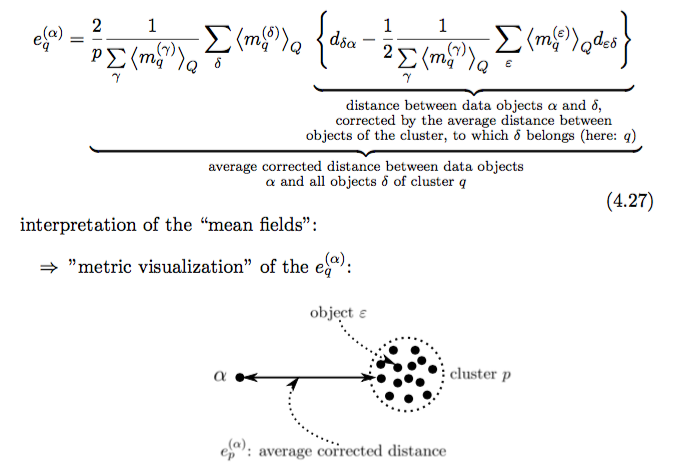
\includegraphics[width=0.7\textwidth]{figures/cl-mean-field-formular}
  \caption{}
%  \label{fig:cl-annealing-epsilon}
\end{figure}

\begin{figure}[hbt]
	\center
  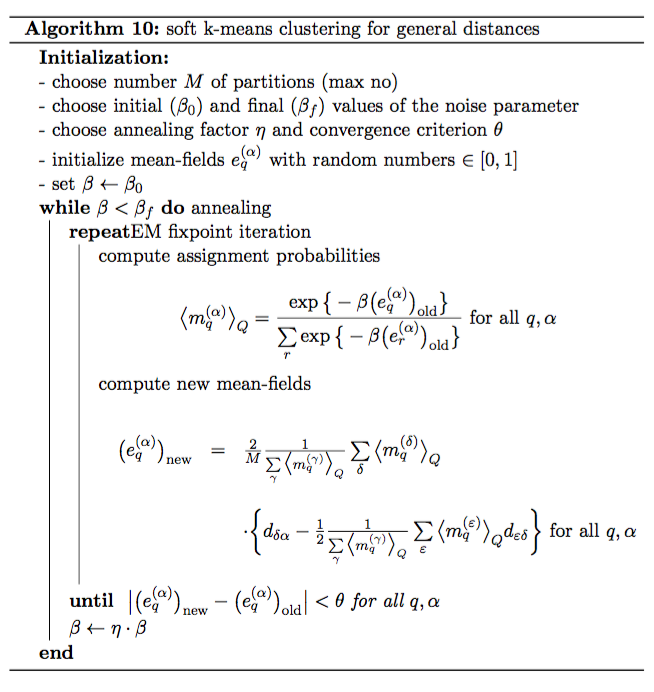
\includegraphics[width=0.5\textwidth]{figures/cl-mean-softkmean-algorithm}
  \caption{}
\end{figure}

\subsection{Missing data}
Sometimes, we don't have access to all $d_{q\alpha}$ pairs. We can derive as follow : 
\begin{align*}
	\bar{d}_{q\alpha} &= \frac{\sum_\gamma \langle m_q^{(\gamma)} \rangle_Q d_{\gamma\alpha} }{ \sum_\gamma \langle m_q^{(\gamma)} \rangle_Q } \\
	e_q^{(\alpha)} &= \Bigg \{  \bar{d}_{q\alpha} - \frac{1}{2} \sum_{\delta} \langle m_q^{(\delta)} \rangle_Q  \bar{d}_{\gamma\delta}\Bigg \}
\end{align*}

Therefore, we can compute $\bar{d}_{\gamma\delta}$ using only measured data that we have.

\subsection{Soft K-means for Euclidean distances}


\begin{align*}
	d_{\alpha\alpha'} &= \frac{1}{2}\bigg(  \boldsymbol{x}^{(\alpha)}  -  \boldsymbol{x}^{(\alpha')} \bigg)^2 \\
	e_q^{(\alpha)} &= \frac{1}{2}\bigg(  \boldsymbol{x}^{(\alpha)}  -  \boldsymbol{w}_q \bigg)^2
\end{align*}
and 
$$
\boldsymbol{w}_q = \frac{ \sum_\gamma \langle m_q^{(\gamma)} \rangle_Q \boldsymbol{x}^{(\gamma)} }{ \sum_\gamma \langle m_q^{(\gamma)} \rangle_Q }
$$

\begin{figure}[hbt]
	\center
  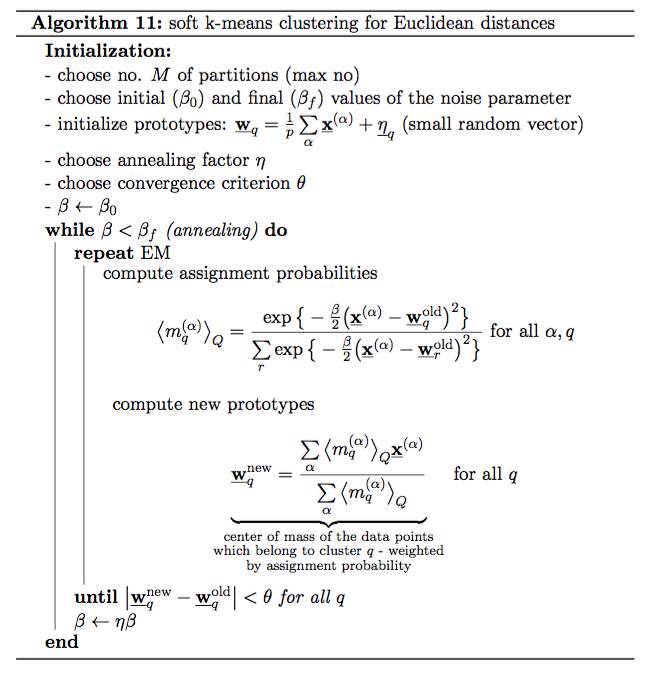
\includegraphics[width=0.5\textwidth]{figures/cl-soft-k-mean-eucli}
  \caption{Soft K-means with Euclidean distance}
\end{figure}

For online version, we compute $\langle m_q^{(\alpha)} \rangle_Q , \forall q \in M $ and then update $\boldsymbol{w}_q $ with the rule :
$$
\boldsymbol{w}_q \leftarrow \boldsymbol{w}_q + \eta \langle m_q^{(\alpha)} \rangle_Q \bigg( \boldsymbol{x}^{(\alpha)} -  \boldsymbol{w}_q \bigg) 
$$

\subsection{Influence of $\beta$ to cluster structure}

Average cost is 
$$
\langle E \rangle = \frac{1}{Z} \sum_{ \{ m_p^{(\alpha)} \} } E\exp{ ( -\beta E ) }
$$

$\uparrow \beta$ means $\downarrow $ average cost,  $\downarrow $ cluster size and $\uparrow$ hierachical clustering.

\begin{figure}[hbt]
	\center
  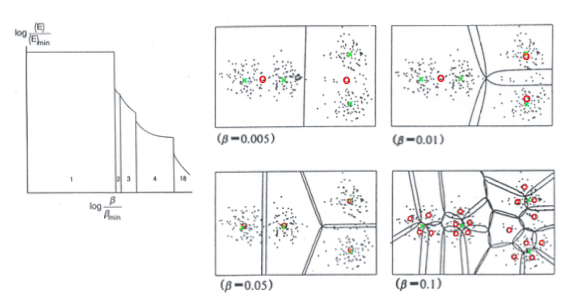
\includegraphics[width=0.5\textwidth]{figures/cl-beta-cluster}
  \caption{Influence of $\beta$ to cluster structure}
\end{figure}

\begin{figure}[hbt]
	\center
  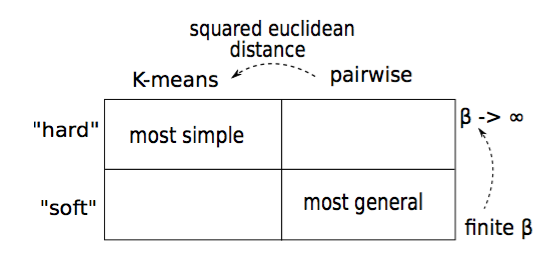
\includegraphics[width=0.5\textwidth]{figures/cl-summary}
  \caption{Summary of clustering algorithms}
\end{figure}

\section{Self-Organizing Maps(SOM)}
SOM is a clustering algorithm that is based on similarity, e.g. Euclidean distance. It's a low-dimensional embedding technique that preverves neighborhood.


\begin{algorithm}[H]
\caption{On-line learning for SOM}
 \KwData{ choose of no. partitions ( clusters ) $M$}
 \KwData{ choose of annealing schedule $\epsilon$ and $\sigma$ }
 \For{$\alpha = \text{shuffle}(\{1,\dots, p \})$}{
 Find the closest prototype : $p = \underset{r}{\text{argmin}} | \boldsymbol{x}^{(\alpha)} - \boldsymbol{w}_r | $
 
$\forall q$ : update $\boldsymbol{w}_q$ respect to :
 \begin{align*}
 	h_{qp}  &= \exp{ \bigg (  - \frac{(p-q)^2}{2\sigma^2} \bigg) } \tag*{(Neighborhood function)} \\
 	\Delta\boldsymbol{w}_q &= \epsilon h_{qp} ( \boldsymbol{x}^{(\alpha)} - \boldsymbol{w}_q ) 
 \end{align*}
 }
\end{algorithm}

Noting that, if $\sigma = 0$ the algorithm becomes an standard on-line K-means.

\subsection{Neighborhood function $h_{qp}$}
\begin{align*}
	h_{qp}  &= \exp{ \bigg (  - \frac{(p-q)^2}{2\sigma^2} \bigg) } 
\end{align*}
\begin{itemize}
	\item $\uparrow \sigma$ gives us smooth cost function $\implies$ lower-cost optimization but results might not well represent the data.
	\item $\downarrow \sigma$ gives us rough cost function $\implies$ higher-cost optimization but has more representation capabilities.
\end{itemize}

\subsection{Self-organizing maps for pairwise data}
\begin{itemize}
	\item For each pair of data, we compute dissimilarity $d_{\alpha\alpha'}$.
	\item Construct $M$ clusters with geometrical structure ( 1d line, 2d grid )
	\item $m_q^{(\alpha)}$ binary assignment variable ( normalize to 1 for each $\alpha$ )
$$
m_q^{(\alpha)} = \text{1}\{  \boldsymbol{x}^{(\alpha)} \ \text{ belongs to } \ \boldsymbol{w}_q \}
$$
\end{itemize}
\subsubsection{Cost Function}

\begin{align*}
	E_{ [ \{ m_{q}^{(\alpha)} \} ] } &=  \frac{1}{p} \sum_r \frac{ \sum_{\alpha,\alpha'} \bigg (\sum_q h_{rq} m_q^{(\alpha)} \bigg ) \bigg (\sum_q h_{rq} m_q^{(\alpha')} \bigg ) d_{\alpha\alpha'} }{ \sum_\alpha \bigg (\sum_q h_{rq} m_q^{(\alpha)} \bigg ) } \\
	&\stackrel{!}{=} \min
\end{align*}
This cost function is similar to pairwise clustering but $\boldsymbol{w}_q$ is replaced by $\sum_q h_{rq} m_q^{(\alpha)}$.

\begin{figure}[hbt]
	\center
  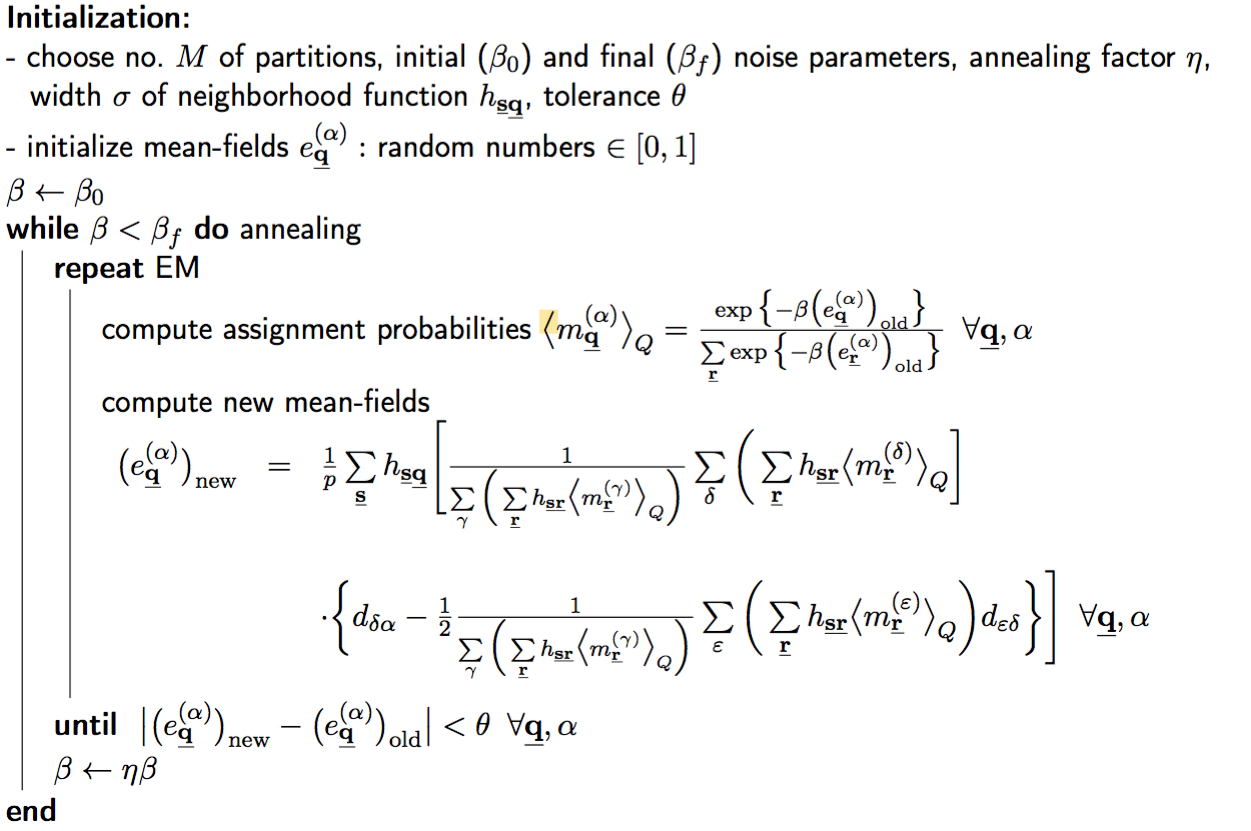
\includegraphics[width=0.7\textwidth]{figures/cl-som-pairwise}
  \caption{SOM for Pairwise data with mean-field approximation}
  \label{fig:cl-som-pairwise}
\end{figure}

From Figure \ref{fig:cl-som-pairwise}, if we replace $h_{qp}$ with Direc's $\delta_{qp} = 1\{ q = p \}$, the computation becomes standard pairwise clustering. This is called "Kohonen-approximation", hence no need $\sigma$  for annealing.

\subsubsection{Euclidean distances}
$$
d_{\alpha\alpha'} = \frac{1}{2} \bigg ( x^{(\alpha)} - x^{(\alpha')} \bigg )^2
$$

\begin{align*}
	E_{[ \{ m_q^{(\alpha)} \} ]} &= \frac{1}{p} \sum_{q,\alpha} \bigg (\sum_p h_{qp} m_p^{(\alpha)} \bigg ) ( \boldsymbol{x}^{(\alpha)} - \boldsymbol{w}_q)^2 \\
	&= \frac{1}{p} \sum_{p,\alpha} m_p^{(\alpha)} \bigg ( \sum_q h_{qp}  \bigg ) ( \boldsymbol{x}^{(\alpha)} - \boldsymbol{w}_q)^2 \\
	\boldsymbol{w}_q  &= \frac{\sum_{\alpha'}\bigg ( \sum_p h_{qp} m_p^{(\alpha')} \boldsymbol{x}^{(\alpha')} \bigg)  }{\sum_{\alpha'}\bigg ( \sum_p h_{qp} m_p^{(\alpha')} \bigg )}
\end{align*}

$\boldsymbol{w}_q$ is now a center of mass of the cluster weighted by neighborhood function $h_{qp}$.

\begin{algorithm}[H]
\caption{On-line learning for SOM with Euclidean distances}
 \KwData{ choose of no. partitions ( clusters ) $M$}
 \KwData{ choose of annealing schedule $\epsilon$}
 \For{$\alpha = \text{shuffle}(\{1,\dots, p \})$}{
 Find the closest prototype : $p = \underset{r}{\text{argmin}} \sum_q h_{rq} ( \boldsymbol{x}^{(\alpha)} - \boldsymbol{w}_q )^2 $
 
$\forall q$ : update $\boldsymbol{w}_q$ respect to :
 \begin{align*}
 	h_{qp}  &= \exp{ \bigg (  - \frac{(p-q)^2}{2\sigma^2} \bigg) } \tag*{(Neighborhood function)} \\
 	\Delta\boldsymbol{w}_q &= \epsilon h_{qp} ( \boldsymbol{x}^{(\alpha)} - \boldsymbol{w}_q ) 
 \end{align*}
 }
\end{algorithm}

\section{Locally Linear Embedding}

Locally linear embedding (LLE) seeks a lower-dimensional projection of the data which preserves distances within local neighborhoods - quoted from scikit-learn\footnote{http://scikit-learn.org/stable/modules/manifold.html\#locally-linear-embedding}.

Given data $\boldsymbol{x}^{(\alpha)}  \in \mathbb{R}^N, \alpha = \{1, \dots, p \}$.
\begin{enumerate}
	\item Find $K$-nearest neighbors of $\boldsymbol{x}^{(\alpha)}$
	\item Calculate reconstruction weights $W$ of $\boldsymbol{x}^{(\alpha)}$ from its $K$-neighbors.
	\item Obtain embedding $\boldsymbol{u}^{(\alpha)} \in \mathbb{R}^M, M \ll N$ from $W$ and its neighbors' embedding.
\end{enumerate}

\subsection{Find $K$-nearest neighbors}
Traditional $K$-nearest neighbors approach has $O(Np^2)$ complexity, but k-d tree reduces the complexity to $O(Np \log p)$.
\subsection{Calculate  reconstruction weights}
We want to find $W$ that minimizes reconstruction cost 
\begin{align*}
E(\boldsymbol{W}) &= \sum_{\alpha=1}^{p}  \bigg ( \boldsymbol{x}^{(\alpha)} - \sum_{\beta = 1 }^p W_{\alpha \beta } \boldsymbol{x}^{(\beta)} \bigg )^2	\\
&\stackrel{!}{=} \min 
\end{align*}
s.t. 
\begin{align*}
	W_{\alpha\beta} &= 0 \ \text{if} \ \boldsymbol{x}^{(\beta)} \not\in \text{KNN}(\boldsymbol{x}^{(\alpha)}) \\
	\sum_{\beta} W_{\alpha\beta} &= 1
\end{align*}

Nothing that $\boldsymbol{W}$ is asymmetric sparse matrix that have up to $K$ nonempty elements for each row. It is also invariant to linear transformations e.g. rotation, scaling and translation.

For each $\boldsymbol{x}^{(\alpha)}$, 
\begin{itemize}
	\item compute $\boldsymbol{C}^{(\alpha)} \in \mathbb{R}^{K,K}$
	$$
	C^{(\alpha)}_{ij}  =  (\boldsymbol{x}^{(\alpha)} - \boldsymbol{x}^{(\beta_i)})^T(\boldsymbol{x}^{(\alpha)} - \boldsymbol{x}^{(\beta_j)})
	$$
	where $\boldsymbol{x}^{(\beta_i)}, \boldsymbol{x}^{(\beta_j)} \in \text{KNN}(\boldsymbol{x}^{(\alpha)})$
	\item solve linear system
	$$
	\boldsymbol{C}^{(\alpha)} \boldsymbol{\widetilde{w}}^{(\alpha)} = (1,\dots,1)^T
	$$
	\item rescale weight 
	$$W_{\alpha\beta_i} = \frac{ \boldsymbol{\widetilde{w}}_i^{(\alpha)}}{\sum_{j=1}^{K} \boldsymbol{\widetilde{w}}_j^{(\alpha)}} $$
\end{itemize}

\subsection{Obtain Embedding}
We want to find embedding $\forall \alpha \in \{1, \dots, p \}, \boldsymbol{u}^{(\alpha)} \in \mathbb{R}^{M}$ s.t. 

\begin{align*}
	F(\boldsymbol{U}) &= \sum_{\alpha=1}^p \bigg ( \boldsymbol{u}^{(\alpha)} - \sum_{\beta=1}^{p} W_{\alpha\beta} \boldsymbol{u}^{(\beta)} \bigg ) \\
	% TODO : show how to derive F(U)
	&= \sum_{\alpha, \beta=1}^p g_{\alpha\beta} (\boldsymbol{u}^{(\alpha)})^T \boldsymbol{u}^{(\beta)} \\
	&\stackrel{!}{=} \min 
\end{align*}

s.t.
\begin{align*}
	\sum_{\alpha=1}^{p} \boldsymbol{u}^{(\alpha)} &= 0 \tag*{(remove translation)} \\
	\frac{1}{p} \sum_{\alpha=1}^{p} (\boldsymbol{u}^{(\alpha)})^T \boldsymbol{u}^{(\alpha)} &= I \tag*{(prevent trivial solutions e.g. $\boldsymbol{u}^{(\alpha)} = 0$ )}
\end{align*}
where $g_{\alpha\beta} = \delta_{\alpha\beta} - \boldsymbol{W}_{\alpha\beta} - \boldsymbol{W}_{\beta\alpha} + \sum_{\gamma=1}^{p} \boldsymbol{W}_{\gamma\alpha} \boldsymbol{W}_{\gamma\beta}$. 

Equivalently,
\begin{align*}
	\boldsymbol{G} &\in \mathbb{R}^{p,p} \\
	&= \{ g_{\alpha\beta} \} \ , \forall \alpha,\beta = \{1,\dots,p\} \\
	&= (I - W^T) (I-W)
\end{align*}

The solution to $F(\boldsymbol{U})$ is to compute eigen value decomposition of $\boldsymbol{G}$ with $M+1$ from the lowest eigen values. We discard eigen vector $e_p$ whose eigen value is zero. 

\begin{align*}
	\boldsymbol{U} = \begin{pmatrix}
 	e_{p-M}^T \\
 	\cdots \\
 	e_{p-1}^T
 	\end{pmatrix} 
 	= \begin{pmatrix}
 		u^{(1)}, \dots, u^{(p)}
 	\end{pmatrix} \in \mathbb{R}^{M,p}
\end{align*}

\begin{figure}[hbt]
	\center
  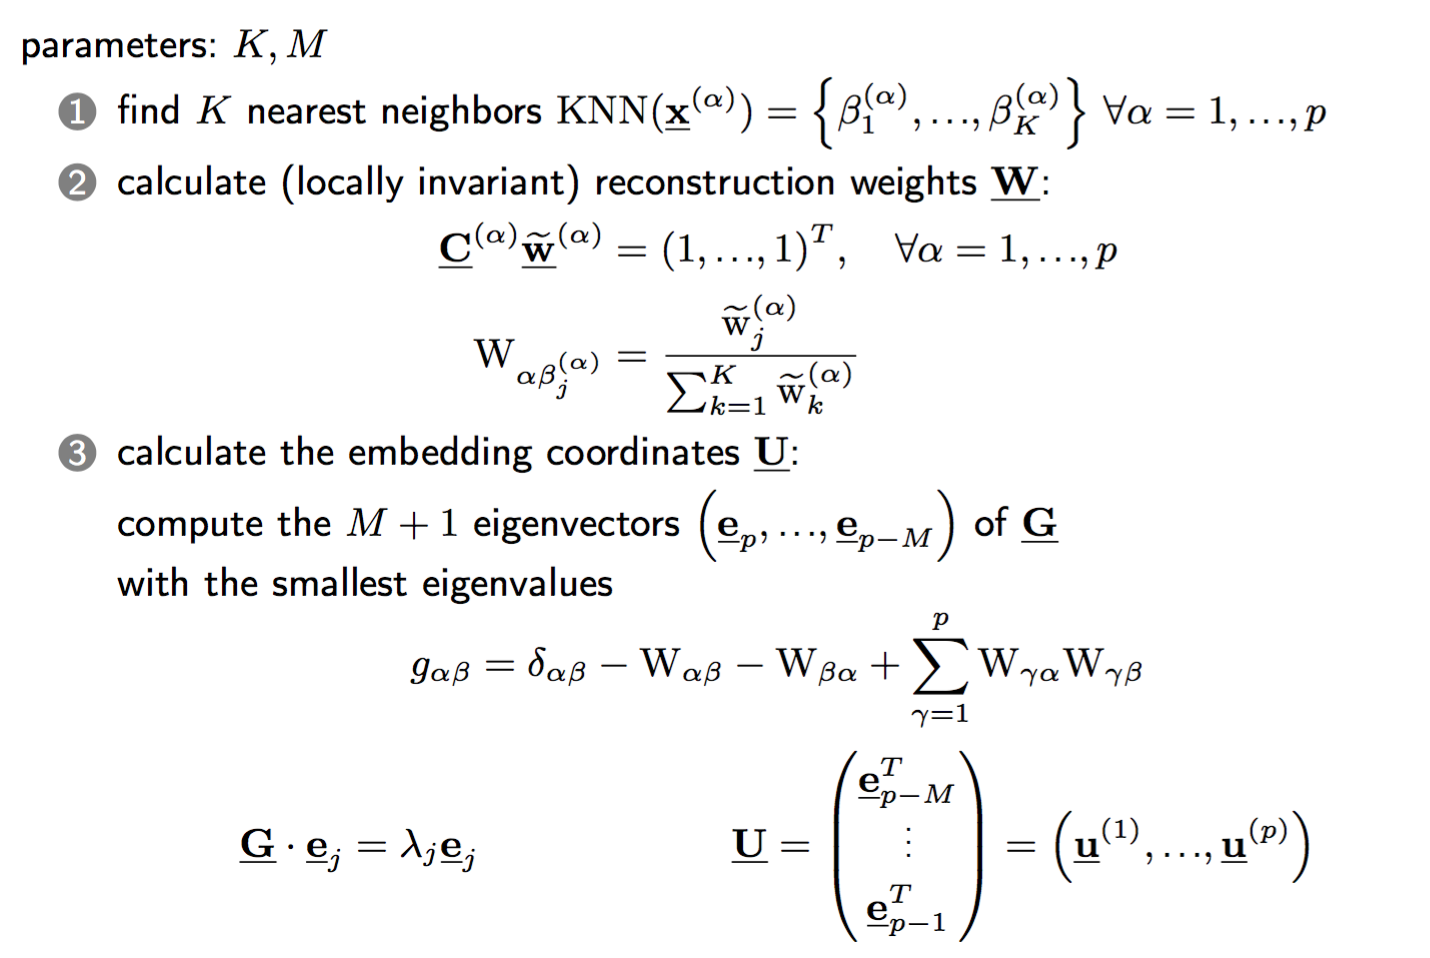
\includegraphics[width=0.5\textwidth]{figures/cl-lle-algo}
  \caption{Locally Linear Embedding Algorithm}
  \label{fig:cl-lle-algo}
\end{figure}
